\documentclass{exam}
\usepackage{pst-eucl}
\usepackage{graphicx} 
\usepackage{changepage, amsmath, amssymb, pgfplots, tikz}
\usetikzlibrary{fit,positioning}
\usepgfplotslibrary{groupplots}
\psset{PointName=none,PointSymbol=none}
\usetikzlibrary{arrows.meta}	
\usetikzlibrary{calc,patterns,angles,quotes}
\pgfplotsset{compat=1.16}
\usetikzlibrary{arrows.meta}
\usepackage{fullpage}
\usepackage{ulem}
\usepackage{tabularx}
\usetikzlibrary{calc,arrows.meta}
\usepackage[most]{tcolorbox}
\definecolor{p1}{HTML}{caf0f8}
\definecolor{p2}{HTML}{ade8f4}
\definecolor{p3}{HTML}{90e0ef}
\definecolor{p4}{HTML}{48cae4}
\definecolor{p5}{HTML}{00b4d8}
\definecolor{p6}{HTML}{0096c7}
\definecolor{p7}{HTML}{0077b6}
\definecolor{p8}{HTML}{023e8a}
\definecolor{p9}{HTML}{03045e}
\usepackage{multicol}
\usepackage{colortbl}
\colorlet{xcol}{blue!60!black}
\usepackage{capt-of}
\definecolor{myred}{HTML}{f44336}
\definecolor{mypink}{HTML}{e81e63}
\definecolor{mypurple}{HTML}{9c27b0}
\definecolor{mydeeppurple}{HTML}{673ab7}
\definecolor{myindigo}{HTML}{3f51b5}
\definecolor{myblue}{HTML}{2196f3}
\definecolor{mylightblue}{HTML}{03a9f4}
\definecolor{mycyan}{HTML}{00bcd4}
\definecolor{myteal}{HTML}{009688}
\definecolor{mygreen}{HTML}{4caf50}
\definecolor{mylightgreen}{HTML}{8bc34a}
\definecolor{mylime}{HTML}{cddc39}
\definecolor{myyellow}{HTML}{ffeb3b}
\definecolor{myamber}{HTML}{ffc107}
\definecolor{myorange}{HTML}{ff9800}
\definecolor{mydeeporange}{HTML}{ff5722}
\definecolor{mybrown}{HTML}{795548}
\definecolor{mygray}{HTML}{9e9e9e}
\definecolor{mybluegray}{HTML}{607d8b}
\definecolor{pag}{HTML}{293133}
\usepackage[labelformat=empty]{caption}
\usepackage{mdframed}
\newtcolorbox{qq}[2][]{%
	boxrule=0.75pt,
	sharp corners,  % Square edges
	colframe=white,  % Set the color of the outline
	colback=pag,  % Set the color of the fill
	coltext=white,
	#1,
}

\usepackage{tikz-3dplot}
\usetikzlibrary{3d,backgrounds,intersections}
% small fix for canvas is xy plane at z % https://tex.stackexchange.com/a/48776/121799
\makeatletter
\tikzoption{canvas is xy plane at z}[]{%
	\def\tikz@plane@origin{\pgfpointxyz{0}{0}{#1}}%
	\def\tikz@plane@x{\pgfpointxyz{1}{0}{#1}}%
	\def\tikz@plane@y{\pgfpointxyz{0}{1}{#1}}%
	\tikz@canvas@is@plane}
\makeatother

\usepgfplotslibrary{groupplots}

\tikzset{
	conditional line/.style 2 args={
		/utils/exec={\pgfmathsetmacro{\xcoordA}{#1}},
		/utils/exec={\pgfmathsetmacro{\xcoordB}{#2}},
		insert path={
			\ifdim\xcoordA pt>\xcoordB pt
			(\xcoordA,0) -- (\xcoordB,0)
			\fi
		},
	},
}

\newcommand{\Logo}{
	\begin{tikzpicture}[remember picture,overlay]
		\node at ($(current page.north east) + (-1cm,-1cm)$) {AC};
	\end{tikzpicture}
}

\newcommand{\tmpsection}[1]{}
\let\tmpsection=\section
\renewcommand{\section}[1]{\tmpsection{#1}\hrule\nobreak}


%--------------------------------------------------------------------
\makeatletter
\newenvironment{multichoices}[1][2]{%
	\begin{multicols}{#1}}{%
\end{multicols}}
\makeatother


\newcommand{\framedtext}[1]{%
	\par%
	\noindent\fbox{%
		\parbox{\dimexpr\linewidth-2\fboxsep-2\fboxrule}{#1}%
	}%
}


\tikzset{
	venn box/.style={
		draw=black, very thick, 
		rounded corners=10,
		inner xsep=10pt, inner ysep=15pt, outer ysep=5pt
	},
	venn numbers/.style={
		%    draw,
		inner ysep=0pt,
		align=center
	},
	venn title/.style={
		fill=black, text=white
	}
}

%--------------------------------------------------------------------

% Portrail


\title{Matematica de 2\textdegree}
\date{\today}
\author{Prof. Alejandro Ceccheto}



\begin{document}
	%% School Portrail.
    \maketitle
\begin{center}
	\includegraphics[width=0.1\linewidth]{"../Latzina/unnamed (1)"}
\end{center}
	
	
	
	\pagebreak
	
	\section{Teoria.}
	\Logo
	
	
	
	\begin{center}
		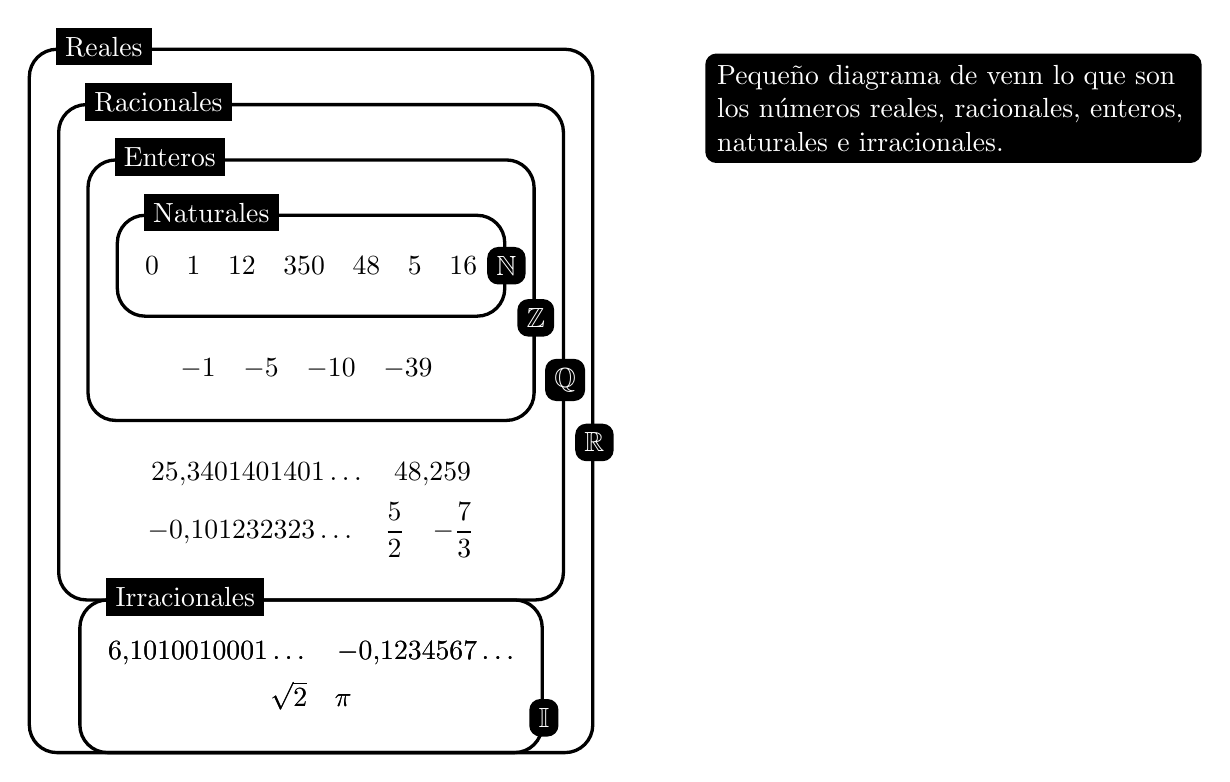
\begin{tikzpicture}[node distance=10pt]
			\node[venn box] (N) {%
				$0 \quad 1 \quad 12 \quad 350 \quad 48 \quad 5 \quad 16$
			};
			
			\node[venn numbers, below=of N] (Z-N) {
				$-1 \quad {-5} \quad {-10} \quad {-39}$
			};
			\node[venn box, fit=(Z-N) (N)] (Z) {};
			
			\node[venn numbers, below=of Z, align=center] (Q-Z) {
				$25{,}3401401401\dots \quad 48{,}259$ \\[5pt]
				$-0{,}101232323\dots \quad \dfrac52 \quad {-\dfrac73}$
			};
			\node[venn box, fit=(Q-Z) (Z)] (Q) {};
			
			\node[venn numbers, below=of Q, inner sep=0pt, align=center] (R-Q) {
				$6{,}1010010001\dots \quad {-0{,}1234567\dots}$ \\[5pt]
				$\sqrt{2} \quad \pi$
			};
			
			\node [venn box, fit=(R-Q) (Q)] (R) {};
			
			% Nuevo nodo para números irracionales
			\node [venn box, fit=(R-Q)] (I) {};
			
			\node[venn numbers, below=of Q, inner sep=0pt, align=center] (R-Q) {
				$6{,}1010010001\dots \quad {-0{,}1234567\dots}$ \\[5pt]
				$\sqrt{2} \quad \pi$
			};
			
			
			
			\tikzset{every node/.style=venn title}
			\foreach \i/\j/\k in {N/Naturales/0, Z/Enteros/10pt, Q/Racionales/10pt, R/Reales/15pt, I/Irracionales/15pt} {
				\draw node[anchor=north west] at ([shift={(10pt, 3pt)}]\i.north west) {\j}
				node[rounded corners] at ([yshift=-\k]\i.east) {$\mathbb{\i}$};
			}
			
			\node at (4,2) [right=1cm,text width=6cm,rounded corners,inner sep=1ex]
			{ Pequeño diagrama de venn lo que son los números reales, racionales, enteros, naturales e irracionales.
			};
		\end{tikzpicture}
	\end{center}

		
		
		
	
	
	
\end{document}